
\section{Mapping cylinders}
\label{sec:mapcyl}


We aim to prove \cref{thm:main_opt_triang}, which says that natural map
\[t_X:DSd\, X\to BX\]
is an isomorphism when $X$ is regular. In this section, we will explain how \cref{thm:main_opt_triang} follows from \cref{thm:barratt_nerve_rep_map_dcr_iso}. At the end of this section, we will make forward references to the work of proving latter.

The skeleton filtration of an arbitrary simplicial set $X$ gives rise to the diagram
\begin{equation}
\label{eq:diagram_mapcyl_skeleton_filtration}
\begin{gathered}
\xymatrix{
DSd\, X^0 \ar[d]^{t_{X^0}} \ar[r] & DSd\, X^1 \ar[d]^{t_{X^1}} \ar[r] & \dots \ar[r] & DSd\, X^n \ar[d]^{t_{X^n}} \ar[r] & \dots \\
BX^0 \ar[r] & BX^1 \ar[r] & \dots \ar[r] & BX^n \ar[r] & \dots
}
\end{gathered}
\end{equation}
and if the vertical maps are all isomorphisms, then $t_X$ is. This is because $t_X$ arises from (\ref{eq:diagram_mapcyl_skeleton_filtration}) as the canonical map between sequential colimits. Next, we explain the latter statement.

Consider the nerve $N:Cat\to sSet$ and the inclusion $U:PoSet\to Cat$. We let the symbol $N$ denote the corestriction to $nsSet$ of the composite $N\circ U$, also. Furthermore, we let $U$ denote the inclusion $U:nsSet\to sSet$. Then $N\circ U=U\circ N$ by definition.

The functor $DSd$ is a left adjoint, so in particular it preserves $X$ viewed as the colimit of its skeleton filtration. Furthermore, the functor
\[(-)^\sharp :sSet\to PoSet\]
is cocontinous, as we explain shortly.

If the inclusion of a full subcategory into the surrounding category has a left adjoint, then we will refer to the subcategory as a \textbf{reflective} subcategory. We then refer to the left adjoint as a \textbf{reflector}. Relevant examples are the facts that $nsSet$ is a reflective subcategory of $sSet$ and that $PoSet$ is a reflective subcategory of $Cat$. Note that the terminology is not standard. Although the fullness assumption seems more common today than before, Mac Lane's notion \cite{ML98}, for example, does not include fullness as an assumption in his definition.

We will also make use of the dual notion. If the inclusion of a full subcategory into the surrounding category has a right adjoint, then we will refer to the subcategory as a \textbf{coreflective} subcategory. Knowing that a subcategory is reflective or coreflective has a bearing on the formation of limits and colimits in the subcategory, as we will point out when it becomes relevant.

The (full) inclusion $U:PoSet\to Cat$ admits a left adjoint $p:Cat\to PoSet$, so $PoSet$ is a reflective subcategory of $Cat$. Furthermore, let $c:sSet\to Cat$ be left adjoint to $N:Cat\to sSet$. Notice that the map $c(b_X)$ gives rise to the map
\[cSd\, X\xrightarrow{c(b_X)} cUBX\xrightarrow{id} cUN(X^\sharp )\xrightarrow{id} cNU(X^\sharp )\xrightarrow{\epsilon _{UX^\sharp }} UX^\sharp\]
that sends the object corresponding to $[x,(\iota )]$ to the object $x$. The $0$-simplex of $Sd\, X$ is here thought of as uniquely represented by a minimal pair $(x,\iota )$ where $x$ is a non-degenerate simplex of $X$ and where $\iota$ is the identity $[n_x]\to [n_x]$ where $n_x$ is the degree of the simplex $x$. The natural map $b_X:Sd\, X\to UBX$ sends the $0$-simplex represented by $(x,(\iota ))$ to the functor $[0]\to X^\sharp$ with $0\mapsto x$.
\begin{lemma}\label{lem:sharp_functor_preserves_colimits}
The functor $(-)^\sharp :sSet\to PoSet$ preserves colimits.
\end{lemma}
\begin{proof}
The map $cSd\, X\to UX^\sharp$ is full and bijective on objects. If we apply posetification $p:Cat\to PoSet$ to the natural map $cSd\, Y\to UY^\sharp$, then we get an isomorphism. This conclusion comes from knowing that $p$ is a reflector. Because $pcSd$ is left adjoint to $ExNU$, where $Ex$ is right adjoint to $Sd$, it follows that $(-)^\sharp$ preserves colimits.
\end{proof}
\noindent This concludes our argument that $(-)^\sharp$ is cocontinous.

The map $t_{X^0}$ is an isomorphism as $b_{X^0}:Sd(X^0)\to B(X^0)$ is, say because $X^0$ is non-singular. Note that the $n$-skeleton $X^n$ can be built from $X^{n-1}$ by successively attaching the non-degenerate $n$-simplices along their boundaries. This building process may be transfinite.
\begin{definition}\label{def:sequence_optriang}
Let $\mathscr{C}$ be a cocomplete category and $\lambda$ some ordinal. A cocontinous functor $Y:\lambda \to \mathscr{C}$ is a \textbf{$\lambda$-sequence} in $\mathscr{C}$. We often write the $\lambda$-sequence as
\[Y^{[0]}\to Y^{[1]}\to \cdots \to Y^{[\beta ]}\to \cdots \]
where $Y^{[\beta ]}=Y(\beta )$ for $\beta <\lambda$. The canonical map $Y^{[0]}\to colim_{\beta <\lambda }Y^{[\beta ]}$ is the \textbf{composition} of $Y$. By a \textbf{sequence} we mean a $\lambda$-sequence for some ordinal $\lambda$.
\end{definition}
\noindent When $\lambda <\aleph _0$ is finite, then the composition of a $\lambda$-sequence is simply the composite of the maps in the sequence.

In the case when one admits $\lambda >\aleph _0$, like we do, one often uses the adjective \emph{transfinite} to indicate this as the term \emph{sequence} usually refers to the notion of $\aleph _0$-sequence. However, we usually admit $\lambda >\aleph _0$ and prefer instead to point it out if the sequence in question is a $\aleph _0$-sequence, whenever it is relevant.

The following highly flexible notion \cite[Def.~10.2.1]{Hi03} will be useful.
\begin{definition}
Let $n$ be some non-negative integer. If a map $f:X\to X'$ is a composition of some sequence $Y$ such that each map $Y^{[\beta ]}\to Y^{[\beta +1]}$ in the sequence is a cobase change of the inclusion $\partial \Delta [n]\to \Delta [n]$, then we say that $f$ is a \textbf{relative $\{ \partial \Delta [n]\to \Delta [n]\}$-cell complex} and we say that $Y$ is a presentation of $f$ as a relative $\{ \partial \Delta [n]\to \Delta [n]\}$-cell complex.
\end{definition}
\noindent If $X$ is a simplicial set, then the inclusion $X^{n-1}\to X^n$ is a relative $\{ \partial \Delta [n]\to \Delta [n]\}$-cell complex. See \cite[Cor.~4.2.4~(ii)]{FP90} and \cite[Prop.~10.2.14]{Hi03}. We will use this fact in our problem reduction below, stated as \cref{lem:first_reduction}.

For the compatibility between sequences and colimits in the two categories $PoSet$ and $nsSet$, we will use the following result.
\begin{lemma}
\label{lem:inclusion_poset_nsset_preserves_sequential_colimits}
The functor $N:PoSet\to nsSet$ preserves colimits of sequences.
\end{lemma}
\begin{proof}
The functor $U:PoSet\to Cat$ preserves colimits of sequences \cite[p.~216]{Ra10}. So does $N:Cat\to sSet$, as is well known. By \cref{lem:filtered_colimits_preservation}, the inclusion $U:nsSet\to sSet$ also preserves colimits of sequences. Because $nsSet$ is a reflective subcategory of $sSet$, the counit of the adjunction $(D,U)$ is in general an isomorphism. As $N\circ U=U\circ N$, it follows that $N:PoSet\to nsSet$ preserves colimits of sequences.
\end{proof}
\noindent Remember the non-standard notion of sequence from \cref{def:sequence_optriang}.

By the naturality of $t_X$, because $(-)^\sharp$ is cocontinous by \cref{lem:sharp_functor_preserves_colimits} and because $N$ preserves colimits of sequences by \cref{lem:inclusion_poset_nsset_preserves_sequential_colimits}, it follows that $t_X$ arises from (\ref{eq:diagram_mapcyl_skeleton_filtration}) as a map of sequential colimits. Thus $t_X$ is an isomorphism if $t_{X^n}$ is an isomorphism for each $n\geq 0$.

For our first problem reduction we will also need the following terms, which have a connection with properties of the Barratt nerve.
\begin{definition}
Suppose $\mathscr{B}$ a small category. Let $\mathscr{A}$ be a subcategory of $\mathscr{B}$. We will say that $\mathscr{A}$ is a \textbf{(co)sieve} in $\mathscr{B}$ if whenever we have a morphism $b\to b'$ whose target (source) is an object of $\mathscr{A}$, then the morphism is itself a morphism of $\mathscr{A}$.
\end{definition}
\begin{lemma}\label{lem:first_reduction}
The natural map $t_X:DSd\, X\to BX$ is an isomorphism whenever $X$ is regular if it is an isomorphism for each regular $X$ that is generated by a single simplex.
\end{lemma}
\begin{proof}
We will use a double induction. Suppose $n>0$ such that $t_X$ is an isomorphism whenever the dimension of $X$ is strictly lower than $n$. This will be our outer induction hypothesis. It is satisfied for $n=1$.

As our inner induction hypothesis, suppose $\lambda >0$ an ordinal such that a regular simplicial set $X$ has the property that $t_X$ is an isomorphism whenever the inclusion $X^{n-1}\to X$ can be presented by some $\gamma$-sequence
\[X^{n-1}=Y^{[0]}\to Y^{[1]}\to \cdots \to Y^{[\beta ]}\to \cdots \]
with $\gamma <\lambda$ as a relative $\{ \partial \Delta [n]\to \Delta [n]\}$-cell complex. The hypothesis is satisfied for $\lambda =1$ by the outer induction hypothesis.

Suppose $X$ a regular simplicial set such that the inclusion $X^{n-1}\to X$ can be presented by some $\lambda$-sequence $Y:\lambda \to sSet$ a relative $\{ \partial \Delta [n]\to \Delta [n]\}$-cell complex.

The case when $\lambda$ is a limit ordinal is handled by the same argument as the one concerning (\ref{eq:diagram_mapcyl_skeleton_filtration}).

Consider the case when $\lambda =\beta +1$ is a successor ordinal. Then $Y^{[\beta ]}$ is the colimit of a $\beta$-sequence, so $t_{Y^{[\beta ]}}$ is an isomorphism by the inner induction hypothesis. We shift notation and write $X'=Y^{[\beta ]}$ and $X=Y^{[\beta +1]}$. Thus we study an attaching
\[X=\Delta [n]\sqcup _{\partial \Delta [n]}X',\]
meaning the regular simplicial set $X$ is built from $X'$ by attaching some non-degenerate $n$-simplex $x$.

In general, the Barratt nerve behaves badly when applied to pushouts, so we choose a different decomposition of $X$ that the Barratt nerve respects. The decomposition that we have in mind, which is used for the same purpose in the proof of \cite[Prop.~2.5.8]{WJR13}, does not depend on regularity, although $X$ is regular.

Let $Y$ denote the simplicial subset of $X$ that is generated by $x$, or in other words, the image of its representing map $\bar{x} :\Delta [n]\to X$. If we take the pullback $Y'$ along the inclusion $X'\to X$, then we get a diagram
\begin{displaymath}
\xymatrix{
\partial \Delta [n] \ar[dd] \ar@{-->}[dr] \ar[rr] && X' \ar[dd] \\
& Y' \ar[dd] \ar[ur] \\
\Delta [n] \ar[dr] \ar@{-}[r]^(.65){\bar{x} } & \ar[r] & X \\
& Y \ar[ur]
}
\end{displaymath}
that gives rise to a factorization
\[X\to Y\sqcup _{Y'}X'\to X\]
of the identity. Furthermore, the map $Y\sqcup _{Y'}X'\to X$ is degreewise injective. Hence the simplicial set $X$ can be viewed as the pushout $Y\sqcup _{Y'}X'$.

Inductively, we can assume that $t_{Y'}$ is an isomorphism, so we have the diagram
\begin{displaymath}
\xymatrix{
DSd\, Y \ar[d]_{t_Y} & DSd\, Y' \ar[l] \ar[d]_{t_{Y'}}^\cong \ar[r] & DSd\, X' \ar[d]_{t_{X'}}^\cong \\
B\, Y & B\, Y' \ar[l] \ar[r] & B\, X'
}
\end{displaymath}
giving rise to a map between pushouts in $nsSet$ that $t_X$ factors through, by naturality. In fact, the Barratt nerve preserves the pushout $Y\sqcup _{Y'}X'$ as we explain in the next paragraph.

The sharp functor $(-)^\sharp :sSet\to PoSet$ is cocontinous by \cref{lem:sharp_functor_preserves_colimits}, so
\[X^\sharp =Y^\sharp \sqcup _{(Y')^\sharp}(X')^\sharp.\]
Moreover, $(-)^\sharp$ turns degreewise injective maps into sieves by \cref{lem:sharp_creates_sieves}. This means that the square
\begin{displaymath}
\xymatrix{
	U((Y')^\sharp ) \ar[d] \ar[r] & U((X')^\sharp ) \ar[d] \\
	U(Y^\sharp ) \ar[r] & U(X^\sharp )
}
\end{displaymath}
is cocartesian in $Cat$ \cite[p.~315]{Th80}. It is readily checked that the latter cocartesian square is preserved by $N:Cat\to sSet$ \cite[p.~315]{Th80}. Thus the Barratt nerve $B:sSet\to sSet$ preserves the pushout $X=Y\sqcup _{Y'}X'$. It follows that $t_X$ is an isomorphism if $t_Y$ is.

Note that $Y$ is generated by an $n$-simplex, by definition. We shift back to the previous notation $Y^{[\beta ]}=X'$ and $Y^{[\beta +1]}=X$. Namely, we have proven that $t_{Y^{[\beta +1]}}$ is an isomorphism given that $t_{Y^{[\beta ]}}$ is, and given the assumption of \cref{lem:first_reduction} that $t_X$ is an isomorphism whenever $X$ is regular and generated by a single simplex. This concludes the inner induction.

Let $X$ be some regular simplicial set of dimension $n$, meaning $X=X^n$. It follows from the outer induction hypothesis that $t_{X^{n-1}}$ is an isomorphism. By the inner induction, we know that $t_{X^n}$ is an isomorphism. It follows from the considerations concerning (\ref{eq:diagram_mapcyl_skeleton_filtration}) that $t_X$ is an isomorphism for every regular simplicial set $X$ given the assumption of \cref{lem:first_reduction}. Namely, the combination of \cref{lem:sharp_functor_preserves_colimits} and \cref{lem:inclusion_poset_nsset_preserves_sequential_colimits} shows that $t_X$ arises as a map between colimits of sequences from (\ref{eq:diagram_mapcyl_skeleton_filtration}).
\end{proof}
\noindent The purpose of reducing the proof that $t_X$ is an isomorphism for regular $X$ to the case when $X$ is generated by a single simplex is that we can then take advantage of a technique due to Thomason \cite{Th80}. This technique will reduce our problem further to its technical core, similar to how the use of mapping cylinders can be used in problem reduction. In fact, mapping cylinders is a special case and they show up in our argument.

The following definition of Thomason's \cite{Th80} has been adjusted to suit our needs, but in the restricted context of posets it is equivalent to the original one.
\begin{definition}[Thomason]\label{def:dwyer_map}
Let $k:P\to Q$ be a functor between posets $P$ and $Q$. We will say that $k$ is a \textbf{Dwyer map} if it embeds $P$ as a sieve in $Q$ and if there is a factorization
\begin{equation}
\label{eq:diagram_def_dwyer_map}
\begin{gathered}
\xymatrix{
P \ar[dr]_i \ar[rr]^k && Q \\
& W \ar[ur]_j
}
\end{gathered}
\end{equation}
such that $j$ a cosieve and such that $i$ embeds $P$ is a coreflective subcategory of $W$.
\end{definition}
\noindent That $P$ is a coreflective subcategory is to say that $i$ admits a right adjoint $r:W\to P$. The unit $a\to ri(a)$ is then an isomorphism in the poset $W$, which implies that it is an identity as there is no isomorphism in a poset, except the identities. In other words, $r$ is automatically a retraction. In turn, we get that the counit $\epsilon _w$ is the identity for $w=i(a)$.

By \cref{lem:first_reduction} we are left with proving \cref{prop:t_X_iso_when_X_regular_gen_single_simplex} below, in order to deduce \cref{thm:main_opt_triang}. \cref{prop:t_X_iso_when_X_regular_gen_single_simplex} can be proven from \cref{thm:barratt_nerve_rep_map_dcr_iso} by induction on the degree of the non-degenerate simplex that generates $X$.

The induction step is handled by the following lemma, which reduces our problem to a problem involving mapping cylinders, namely \cref{thm:barratt_nerve_rep_map_dcr_iso}.
\begin{lemma}\label{lem:second_reduction}
Suppose $X$ a regular simplicial set that is generated by a non-degenerate $n$-simplex $x$. Let $y=x\delta _n$. Then $X$ is decomposed by a cocartesian square
\begin{displaymath}
\xymatrix{
\Delta [n-1] \ar[d]_{N\delta _n} \ar[r]^(.6){\bar{y} } & Y \ar[d] \\
\Delta [n] \ar[r]_{\bar{x} } & X
}
\end{displaymath}
in $sSet$. Assume that $t_Y$ is an isomorphism.

Denote $P=\Delta [n-1]^\sharp$ and $Q=\Delta [n]^\sharp$. The map $(N\delta _n)^\sharp$ has a factorization $P\to W\to Q$ that satisfies the condition of being a Dwyer map. The pushouts $W\sqcup _PY^\sharp$ and $Q\sqcup _PY^\sharp$ in $Cat$ are a posets, so $N(W\sqcup _PY^\sharp )$ and $N(Q\sqcup _PY^\sharp )$ are non-singular. Furthermore, \dots
\begin{enumerate}
\item{\dots the map $t_X:DSd\, X\to BX$ is an isomorphism if the canonical map
\[D(NQ\sqcup _{NP}N(Y^\sharp ))\to N(Q\sqcup _PY^\sharp )\]
is an isomorphism. Finally, \dots }
\item{\dots the map $D(NQ\sqcup _{NP}N(Y^\sharp ))\to N(Q\sqcup _PY^\sharp )$ is an isomorphism if
\[D(NW\sqcup _{NP}N(Y^\sharp ))\to N(W\sqcup _PY^\sharp )\]
is an isomorphism.}
\end{enumerate}
\end{lemma}
\noindent The proof of \cref{lem:second_reduction} is deferred to \cref{sec:red}.

What is the announced connection with mapping cylinders? We now explain this. The structure of $(N\delta _n)^\sharp :P\to Q$ as a Dwyer map that we refer to in \cref{lem:second_reduction} is the factorization
\begin{equation}
\label{eq:zeroth_diagram_proof_lem_second_reduction}
\begin{gathered}
\xymatrix{
P \ar[dr]_{i_0} \ar[rr]^{N(\delta _n)^\sharp } && Q \\
& W=P\times [1] \ar[ur]_\psi
}
\end{gathered}
\end{equation}
in which $\psi$ is defined as follows. The function $\psi$ sends the pair
\[(\mu :[m]\to [n-1],0)\]
to the composite
\[[m]\xrightarrow{\mu } [n-1]\xrightarrow{\delta _n} [n],\]
and the pair $(\mu :[m]\to [n-1],1)$ to the face operator
\[[m+1]\to [n]\]
given by $j\mapsto \mu (j)$ for $0\leq j\leq m$ and $m+1\mapsto n$.

Notice that there is only one object of $Q$ that is not in the image of $\psi$, namely the $n$-th vertex $\varepsilon _n:[0]\to [n]$. \cref{fig:Cosieve_in_subdivided_two_simplex_that_contains_second_edge} illustrates the simplicial subset $NW$ of $NQ=B(\Delta [n])$ in the case when $n=2$.

\begin{figure}
\centering
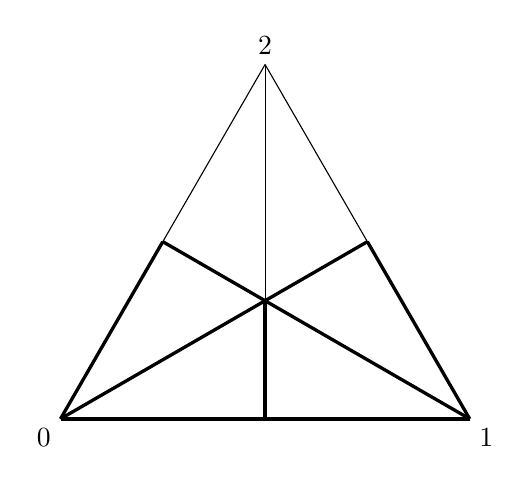
\begin{tikzpicture}

% Vertices of a triangle
\coordinate (2) at (90:3cm);
\coordinate (0) at (210:3cm);
\coordinate (1) at (-30:3cm);

% Nodes to mark vertices of a triangle
\node [above] at (2) {2};
\node [below left] at (0) {0};
\node [below right] at (1) {1};

% Draw line between the vertices 0,1 and 2 and name the midpoints
\draw (0.north east)--(2.south) coordinate[midway](02);
\draw [very thick] (0.north east)--(1.north west) coordinate[midway](01);
\draw (1.north west)--(2.south) coordinate[midway](12);

% Barycenter, could also be found by means of the intersection library of tikz
\coordinate (012) at (barycentric cs:0=1,1=1,2=1);

% Draws lines from vertices of original triangle to barycentre of original triangle and...
\draw [very thick] (0.north east)--(012) coordinate[midway](0<012);
\draw [very thick] (1.north west)--(012) coordinate[midway](1<012);
\draw (2.south)--(012) coordinate[midway](2<012);
\draw [very thick] (01)--(012) coordinate[midway](01<012);
\draw [very thick] (12)--(012) coordinate[midway](12<012); % Illustrate the cosieve
\draw [very thick] (02)--(012) coordinate[midway](02<012); % Illustrate the cosieve

% Illustrate the cosieve
\draw [very thick] (0.north east)--(02);
\draw [very thick] (1.north west)--(12);

\end{tikzpicture}
\caption{Nerve of the cosieve $W$}
\label{fig:Cosieve_in_subdivided_two_simplex_that_contains_second_edge}
\end{figure}

The pushout $Q\sqcup _PY^\sharp$ in $Cat$ is by the paragraph above taken along a Dwyer map, which implies that it is a poset \cite[Lem.~5.6.4]{Th80}. Furthermore, the pushout $W\sqcup _PY^\sharp$ in $Cat$ is a poset, say because it is taken along a rather trivial Dwyer map. Because $PoSet$ is a reflective subcategory of $Cat$ it follows that $W\sqcup _PY^\sharp$ can be considered a pushout in $PoSet$ of the underlying diagram.

Because $W=P\times [1]$, the pushout
\[T(B(\bar{y} ))=NW\sqcup _{NP}N(Y^\sharp )\]
in $sSet$ is the (backwards) topological mapping cylinder of $B(\bar{y} )$. Similarly,
\[M(B\bar{y} ))=N(W\sqcup _PY^\sharp )\]
is the (backwards) reduced mapping cylinder \cite[pp.~56--68]{WJR13}, which was defined in \cref{sec:intro}. Note that the canonical map
\[NW\sqcup _{NP}N(Y^\sharp )\to N(W\sqcup _PY^\sharp ),\]
is a guise of the cylinder reduction map $cr:T(B(\bar{y} ))\to M(B(\bar{y} ))$.

Next, consider the case when $X$ is generated by a single simplex. With the recognition made in the paragraph above, we are ready to discuss this case.
\begin{proposition}
\label{prop:t_X_iso_when_X_regular_gen_single_simplex}
Let $X$ be a regular simplicial set that is generated by a single simplex. Then $t_X$ is an isomorphism.
\end{proposition}
\begin{proof}
We will prove this by induction. Assume that $n>0$ is such that $t_X$ is an isomorphism for any regular $X$ that is generated by a non-degenerate simplex of degree $k<n$.

For the base step, one can note that the hypothesis holds for $n=1$ because $0$-dimensional simplicial sets are non-singular.

For the induction step, we assume that $X$ is as described in \cref{lem:second_reduction} and aim to prove that $t_X$ is an isomorphism. Notice that $Y$ is generated by the non-degenerate part of $y$, which is of degree $n-1$. This means that the assumption that $t_Y$ is an isomorphism, is justified.

\cref{lem:second_reduction} says that it suffices to prove that the map
\[D(NW\sqcup _{NP}N(Y^\sharp ))\to N(W\sqcup _PY^\sharp )\]
from Part $2$ is an isomorphism. In the text preceding this proof we saw that the latter map is a guise of the canonical map
\[dcr:DT(B(\bar{y} ))\to M(B(\bar{y} ))\]
whose source is the desingularized (backwards) topological mapping cylinder.

By \cref{thm:barratt_nerve_rep_map_dcr_iso}, the map $dcr$ is an isomorphism as $Y$ is regular.\\ \cref{lem:second_reduction} thus implies that $t_X$ is an isomorphism. This concludes the induction step.
\end{proof}
\noindent Note that \cref{prop:t_X_iso_when_X_regular_gen_single_simplex} relies upon \cref{thm:barratt_nerve_rep_map_dcr_iso}.

Now, recall \cref{lem:first_reduction}. We are ready to reduce \cref{thm:main_opt_triang} to \cref{thm:barratt_nerve_rep_map_dcr_iso}.
\begin{proof}[Proof of \cref{thm:main_opt_triang}.]
By \cref{prop:t_X_iso_when_X_regular_gen_single_simplex}, the assumption of \cref{lem:first_reduction} is satisfied. Thus we obtain \cref{thm:main_opt_triang}.
\end{proof}
\noindent Next, we keep our promise to explain the structure of the rest of this article.

Like the reader presumably have done so far, he preferably continues to read the sections in order, although there is a small detour in \cref{sec:cones}.

After \cref{sec:red}, which takes care of the deferred proof of \cref{lem:second_reduction}, we focus on \cref{thm:barratt_nerve_rep_map_dcr_iso} whose proof is rather technical. The work of proving \cref{thm:barratt_nerve_rep_map_dcr_iso} is divided into three tasks.

First, in \cref{sec:dzero}, we explain that
\[dcr:DT(B(\bar{y} ))\to M(B\bar{y} ))\]
is a bijection in degree $0$. This is a more or less formal argument involving not much more than the definition of the category $sSet$ as a set-valued functor category and the nerve functor.

Second, in \cref{sec:surject}, we show that $dcr$ is degreewise surjective. This is not trivial, however the answer is in our case more or less to be found in the pre-existing literature.

Third, in \cref{sec:zipping}, we do the part that seems hard to deduce from the literature, namely to prove that $dcr$ is degreewise injective in degrees above $0$. To do this, however, we separate out a few results in sections \ref{sec:tricat} and \ref{sec:deflation_thm}.

Finally, in \cref{sec:comparison}, we deduce \cref{thm:barratt_nerve_rep_map_dcr_iso} from the work of the three sections \ref{sec:dzero}, \ref{sec:surject} and \ref{sec:zipping}.

The reader may consider \cref{sec:cones} on cones as optional, as it is not really part of the storyline. On the other hand, it may yield insights into the idea behind the material in \cref{sec:zipping}. This is because the result presented in \cref{sec:cones} is a precursor. In addition, the reader may prefer our approach to the result stated as \cref{prop:cones_vs_mapping_cylinders} over any known proof.

